% pyrintext.exe test01_pyr.tex
% or
% pyrintext.exe test01_pyr.tex -p ans=0
\documentclass[a4paper]{article}
\setlength{\textwidth}{200mm}
\setlength{\textheight}{280mm}
\setlength{\topmargin}{-18mm}
\usepackage{color}
\usepackage[pdftex]{graphicx}





\begin{document}

	{\Large\bf PyRInText test01} % This is LaTeX line comment

	\begin{enumerate}
		\item {\bf Python example}

			\textless Extended Euclidean Algorithm \textgreater\vspace{1mm}\par
			Given positive integers $a$ and $b$,\par
			find the integer solution $(x, y)$ to $ax+by=gcd(a,b)$, \par
			where $gcd(a,b)$ is the Greatest Common Divisor of $a$ and $b$.
			\begin{enumerate}
				\item 
					$a= 312 ,~b= 534$\par
					solution:~$g(a,~b)=6,~x=12,~y=-7$\par
					$312\times(12)+534\times(-7)=6$
				\item 
					$a= 315 ,~b= 540$\par
					{\color{white}
					solution:~$g(a,~b)=45,~x=-5,~y=3$\par
					$315\times(-5)+540\times(3)=45$}

			\end{enumerate}

		\item {\bf R example}

			\begin{enumerate}
				\item Estimate pi value with Monte Carlo method\par
					estimation of pi value with 
						2003 points = 3.143285
					

					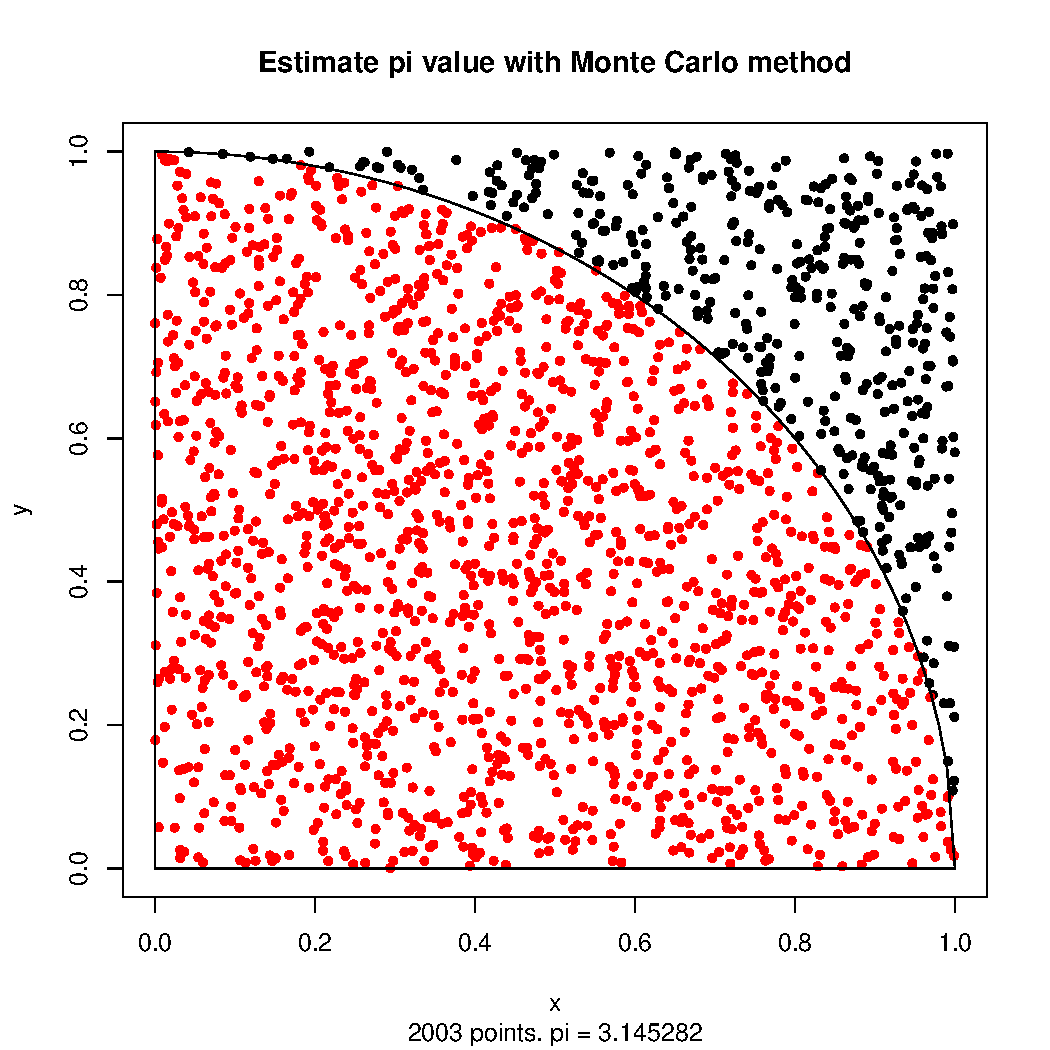
\includegraphics[scale=0.40,clip]{mc_pi.pdf}

				\item IRIS Table using kable\par

					
\begin{tabular}{l|r|r|r|r|l}
\hline
  & Sepal.Length & Sepal.Width & Petal.Length & Petal.Width & Species\\
\hline
41 & 5.0 & 3.5 & 1.3 & 0.3 & setosa\\
\hline
42 & 4.5 & 2.3 & 1.3 & 0.3 & setosa\\
\hline
43 & 4.4 & 3.2 & 1.3 & 0.2 & setosa\\
\hline
44 & 5.0 & 3.5 & 1.6 & 0.6 & setosa\\
\hline
45 & 5.1 & 3.8 & 1.9 & 0.4 & setosa\\
\hline
46 & 4.8 & 3.0 & 1.4 & 0.3 & setosa\\
\hline
47 & 5.1 & 3.8 & 1.6 & 0.2 & setosa\\
\hline
48 & 4.6 & 3.2 & 1.4 & 0.2 & setosa\\
\hline
49 & 5.3 & 3.7 & 1.5 & 0.2 & setosa\\
\hline
50 & 5.0 & 3.3 & 1.4 & 0.2 & setosa\\
\hline
51 & 7.0 & 3.2 & 4.7 & 1.4 & versicolor\\
\hline
52 & 6.4 & 3.2 & 4.5 & 1.5 & versicolor\\
\hline
53 & 6.9 & 3.1 & 4.9 & 1.5 & versicolor\\
\hline
54 & 5.5 & 2.3 & 4.0 & 1.3 & versicolor\\
\hline
55 & 6.5 & 2.8 & 4.6 & 1.5 & versicolor\\
\hline
56 & 5.7 & 2.8 & 4.5 & 1.3 & versicolor\\
\hline
57 & 6.3 & 3.3 & 4.7 & 1.6 & versicolor\\
\hline
58 & 4.9 & 2.4 & 3.3 & 1.0 & versicolor\\
\hline
59 & 6.6 & 2.9 & 4.6 & 1.3 & versicolor\\
\hline
60 & 5.2 & 2.7 & 3.9 & 1.4 & versicolor\\
\hline
\end{tabular}

	
			\end{enumerate}			
	\end{enumerate}
\end{document}

